\begin{figure}[H]
  \centering
  \makebox[\linewidth][l]{\textbf{a}}
  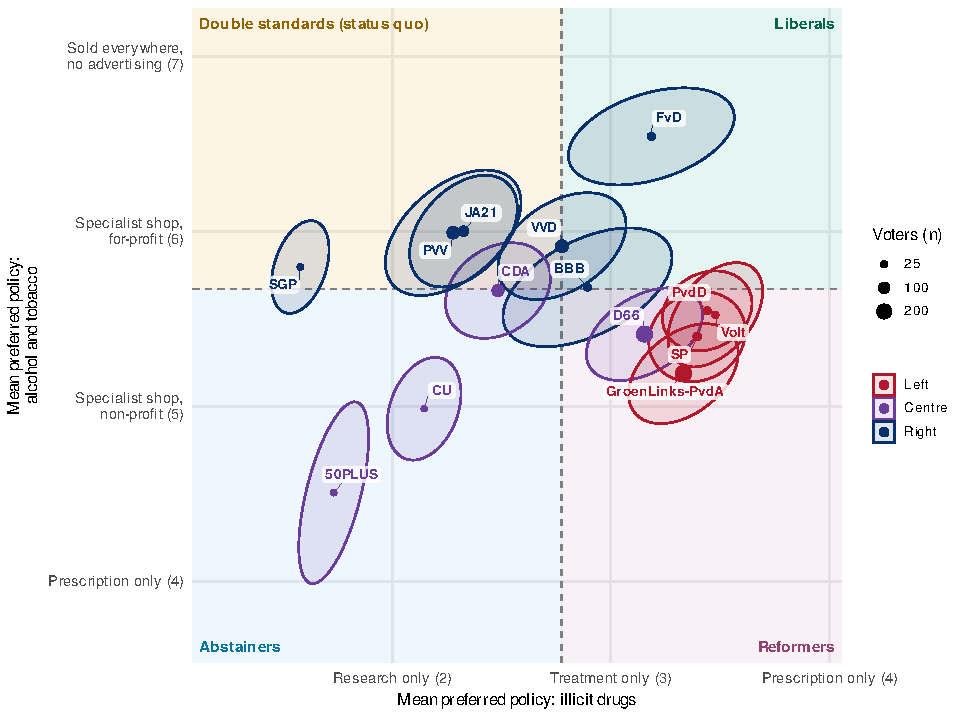
\includegraphics[width=\linewidth]{out/fig_party_map.pdf}\\[4pt]
  \makebox[\linewidth][l]{\textbf{b}}
  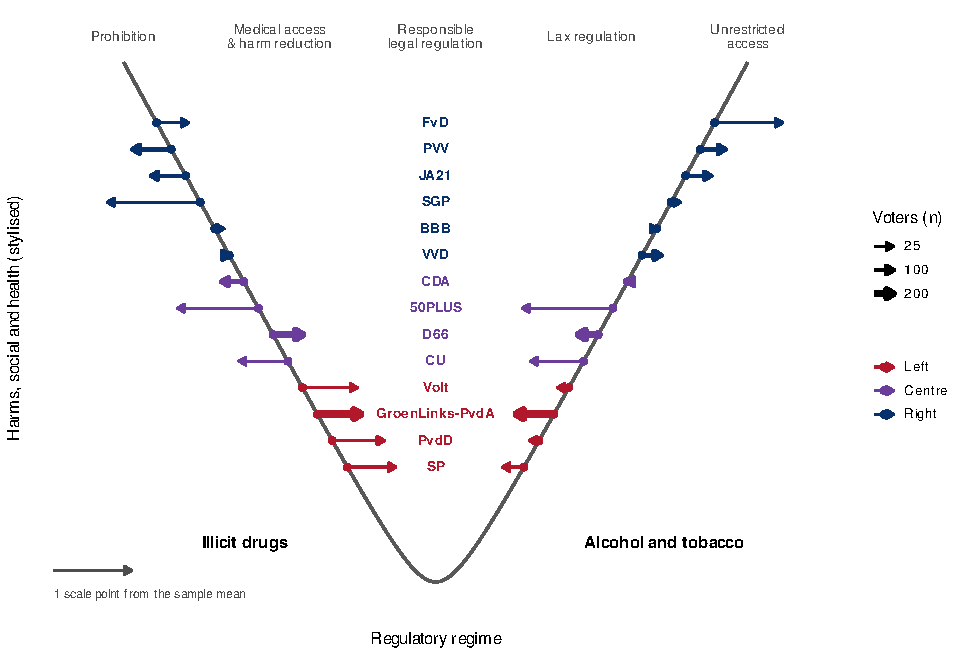
\includegraphics[width=\linewidth]{out/fig_party_map_b.pdf}
  \caption{(a) Parties by the mean preferred policy of their voters for the illicit drugs (horizontal) and for alcohol and tobacco (vertical), from ban (1) to free sale (9). Per respondent the mean answer over the substances answered: horizontal over cannabis, psychedelics, MDMA, speed, cocaine and heroin, vertical over alcohol and tobacco. Dot: the party's weighted mean; ellipse: $\pm 0.2$ standard deviation of its voters (weighted covariance), scaled down so that the parties can be told apart: at full size the ellipses overlap heavily. Their tilt shows the correlation of the two scores within the party. Colour: bloc. Dashed lines are the sample means and split the map into four quadrants: more liberal than average on the legal drugs only (double standards, the status quo), on both (liberals), on neither (abstainers) or on the illicit drugs only (reformers). Point size reflects $n$ ($n = 1153$ in total); DENK ($n = 1$), other parties, blank and non-voters are left out. Vote: TK 2025. (b) The same parties on a stylised U-curve of harms by regulatory regime, after the Transform Drug Policy Foundation. Each party has a row at the same height on both arms, ordered by general left-right (Chapel Hill Expert Survey 2024; right at the top). Each arrow starts on the curve and shows how far, and in which direction, the party's mean differs from the sample mean, in scale points: for the illicit drugs on the left arm, for alcohol and tobacco on the right. Arrow width reflects the number of voters. The heights and start points carry no data; the curve and the regime labels are illustrative.}
  \label{fig:party_map}
\end{figure}
